\chapter{Neural Networks Can Compute Any Function}


This is a condensed write-up of Chapter~4 of Nielsen's book. The objective is 
to present the main ideas of a proof that neural networks can approximate 
any continuous function.

\section{Step Functions and Function Approximation}

There are two main observations in this ``proof.'' First, that a single 
sigmoid neuron can approximate a step function; and second, given 
any interval on the real line $[a, b]$, one can construct a 
fixed-sized network of sigmoid neurons that takes as input a real 
number~$x$ and outputs a $1$ if and only if $x \in (a, b)$. 

It is easy to show that if we want a single sigmoid neuron to step-up 
from $0$ to $1$ at a point~$s$ on the real line, then this can be 
achieved by selecting a high enough weight, say $w = 1000.0$, 
and bias of $b = - s \times w$. This is shown in 
Figure~\ref{fig:nn_step_functions}.
\begin{figure}[ht]
\begin{center}
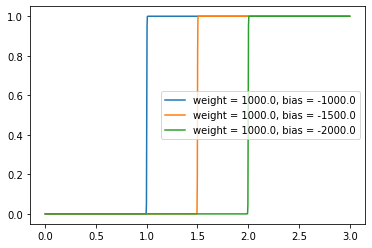
\includegraphics[scale=0.6]{stepfunctions.png}
\end{center}
\caption{Output of a single sigmoid neuron for different values of weight and bias}
\label{fig:nn_step_functions}
\end{figure}

We can now combine two sigmoid neurons which step up at points $s_1$ and $s_2$,
with $s_1 < s_2$, to create a network that outputs a $1$ if and only if $x \in
(s_1, s_2)$ as shown in Figure~\ref{fig:nn_rect_func}. The top neuron of the
hidden layer has a bias $b_1 = - s_1 \times w_1$, where $w_1$ is the weight of
the link between itself and the input node. We choose $w_1$ to be a large
enough number so that this neuron acts as a step function at the point $s_1$.
The bottom neuron in the hidden layer has bias $b_2 = - s_2 \times w_2$, where
$w_2$ is the weight of the link between itself and the input node. As before,
we choose $w_2$ to be large enough so that the bottom neuron steps up at $s_2$. 

Now the trick in making the output of the combined network to be a $1$ when the
input is in the interval $(s_1, s_2)$ is by adjusting the weights of the links
from the hidden layer to the output neuron. We set the weight of the upper link
from the top-most neuron to the output neuron to be $h$ and the weight of the
lower link to be $-h$. Here $h$ is just a very large number. The bias of the
output neuron is set to $-h/2$. The resulting output is then given by:
\[
    \sigma (h \cdot a_1 - h \cdot a_2 - h/2),
\]
where $a_1 = \sigma(w_1 x + b_1)$ and $a_2 = \sigma(w_2 x + b_2)$.
Now $a_1 = 1$ iff $x > s_1$ and $a_2 = 1$ iff $x > s_2$. Thus if $x < s_1$, 
the output is $\sigma(-h/2) \approx 0$; if $x \in (s_1, s_2)$, 
the output is $\sigma(h/2) \approx 1$; 
if $x > s_2$ the output $\sigma(-h/2) \approx 0$. 
At the boundary points, $s_1$ and $s_2$, 
the output is a number between $0$ and $1$. This is because the neurons 
can only approximate a step function. This construct forms the basis 
of how we can approximate arbitrary continuous functions from $\R^m \to \R^n$. 
\begin{figure}[ht]
\begin{center}
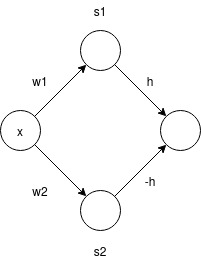
\includegraphics[scale=0.5]{RectFunction.jpg}
\end{center}
\caption{Network of sigmoid neurons to output a rectangle function.}
\label{fig:nn_rect_func}
\end{figure}

\section{Functions of One Variable}

The network described in the last section acts as an indicator function 
for an interval $[s_1, s_2]$ of the real line. Consider a function 
$f \colon \Rone \to \Rone$ whose mean value in the interval $[s_1, s_2]$ 
is $y$. If we were to now weight the output of the network by $y$ by 
adding an extra output node with a linear activation function, the resulting 
output of this new network will be a $y$ whenever $x \in (s_1, s_2)$ and a $0$ 
otherwise. Piecing together several of these networks would allow us 
to output the approximate value of $f$ over several intervals. 
\section{Functions of Several Variables}
